\documentclass[xcolor=table]{beamer}
\usepackage[utf8]{inputenc}

\usepackage[
    backend=biber,
    style=numeric,
    sorting=none
]{biblatex}
\addbibresource{thesis/refs.bib}

\title[Spoof proof GPS timing] % (optional, only for long titles)
{Spoof proof GPS timing}
\subtitle{A detection and mitigation system for GPS time spoofing}
\author[A. Schultzen] % (optional, for multiple authors)
{A.~Schultzen\inst{1}$^{,}$\inst{3}}
\institute[Universities Here and There] % (optional)
{
  \inst{1}%
  Department of Informatics\\
  University of Oslo
  \and
  \inst{3}
  UNIK\\
  University Graduate Center
}
\date[KPT 2004] % (optional)
{Conference on Presentation Techniques, 2004}
\subject{Computer Science}

\date{\today}
\usetheme{Marburg}

\begin{document}
\frame{\titlepage}
\begin{frame}
\frametitle{Agenda}
\section *{Agenda}
\tableofcontents
\end{frame}

\section{Introduksjon}
\begin{frame}
\frametitle{Bruksområder for GPS timing}
	\subsection{Bruksområder for GPS timing}
  GPS timing er timing generert av GPS disiplinerte klokker. Eksempler på bruksområder er:
  \begin{itemize}
    \item Tidsstempling av transaksjoner på Internett .
    \item Fasemålinger i kraftnett.
    \item Telekommunikasjon.
  \end{itemize}
\end{frame}

\subsection{Utfordringer}
\begin{frame}
\frametitle{Utfordringer med GPS timing}
  \begin{itemize}
    \item Avhengig av å ha en antenne med fri sikt.
    \item Kjent kodestruktur.
    \item Naive mottakere.
  \end{itemize}
  GPS basert timing kan derfor ses på som en ukryptert og fysisk usikker kanal inn i mange industrielle kontroll systemer.
\end{frame}

\subsection{Trusler}
\begin{frame}
  \frametitle{Trusler mot GPS timing}
  \begin{itemize}
    \item Jamming. 
    \item Narring.
    \begin{itemize}
      \item Replay.
      \item Data-nivå. 
      \item Signal-nivå.
    \end{itemize}
    \item Feil i utstyr.
  \end{itemize}    
\end{frame}

\subsubsection{Referansenarrer}
\begin{frame}
  \frametitle{"The Civil GPS Spoofer"}
  \begin{figure}
    \includegraphics[scale=0.2]{pics/texas_spoofer.jpg}
    \caption{Civil GPS Spoofer}
  \end{figure}
  "The Civil GPS Spoofer"
  \begin{itemize}
    \item Laget et av et team fra \textit{The University of Texas at Austin} i 2012 \cite{EVPMUGA}
    \item Implementert i SDR
    \item Kan lage opptil 14 "falske" L1 C/A signaler
  \end{itemize}
\end{frame}

\begin{frame}
  \frametitle{"The Civil GPS Spoofer"}
  Nøkkelfunksjoner:
  \begin{itemize}
    \item Sømløs narring, offeret låser på en kopi av det autentiske signalet. Ingen forandring i løsning.
    \item Angriper manipulerer signalet.
    \item Angriperen har gjerne et stort spillerom under angrepet da oscillatoren i mottakeren ofte er av lav kvalitet.
  \end{itemize}
\end{frame}

\section{Mottiltak}
\begin{frame}
\frametitle{Mottiltak}
  \begin{itemize}
    \item Bruke flere GPS mottakere.
    \item Bruke stabil klokke som referanse.
  \end{itemize}
\end{frame}

\subsection{Flere GPS mottakere}
\begin{frame} 
  \frametitle{Bruke flere GPS mottakere}
  Gitt følgende scenario hvor en bruker tre GPS mottakere:
  \begin{itemize}
    \item \textbf{Ingen av mottakerne er narret:} Hver mottakers løste posisjon er lik deres respektive kjente posisjoner. Alle løser samme tid.
    \item \textbf{En eller flere mottakere er narret:} Hvis en mottaker er narret, vil den løse annen tid en de/den som ikke er narret. Er flere enn en men ikke alle narret, vil de narrede også løse samme sted.
    \item \textbf{Alle mottakerne er narret:} Alle mottakerne løser samme posisjon og klokkebias.
  \end{itemize}
\end{frame}

\subsection{Referanseklokke}
\begin{frame}
  \frametitle{Referanseklokke}
  Med en stabil og pålitelig klokke, har en muligheter til å:
  \begin{itemize}
    \item Verifisere GPS løsning.
    \item Realisere nøyaktig timing selv når GPS disiplinering ikke er mulig.
  \end{itemize}
  \begin{columns}
    \column{0.5\textwidth}
      \begin{figure}
        \includegraphics[scale=0.2]{pics/5071A.jpg}
        \caption{Symmetricom 5071A Cesium Primary Frequency Standard (500 000 NOK)}
      \end{figure}
    \column{0.5\textwidth}
      \begin{figure}
        \includegraphics[scale=0.2]{thesis/graphics/csac.jpg}
      \caption{Symmetricom SA.45s CSAC (5000 NOK)}
    \end{figure}
  \end{columns}
\end{frame}

\section{Implementasjon}
\subsection{Krav}
\begin{frame}
  \frametitle{Krav}
  Følgende krav ble identifisert til systemet:
  \begin{itemize}
    \item Kunne detektere at angrep hurtig
    \item Ha mulighet for å logge data
    \item Rask og enkel tilgang til innsamlet data
    \item Ha støtte for mange GPS mottakere
    \item Kunne administreres over nettverk
    \item Konfigurerbar 
  \end{itemize}
\end{frame}

\subsection{Implementasjon}
\begin{frame}
  \frametitle{Atomic Clock Controller Software}
  \begin{itemize}
    \item Klient/Server modell
    \item Filtre
    \item Klokkemodell
    \item Klokkestyring
  \end{itemize}
\end{frame}

\subsubsection{Klient/Server modell}
\begin{frame}
  \frametitle{Klient/Server modell}
  \begin{itemize}
    \item Mottaker + Raspberry PI = Sensor
    \item Antall mottakere begrenset av serverens CPU og RAM
    \item Eliminerer behovet for lange signalkabler, mulig å bruke et vanlig nettverk:
    \begin{itemize}
      \item Fiber
      \item Mobilnett (3G og 4G)
      \item WiFi
    \end{itemize}
  \end{itemize}
\end{frame}

\begin{frame}
\frametitle{Klient/Server modell}
  \begin{itemize}
    \item Klienten kobler til Serveren
    \item Klienten sender utvalgt NMEA (GPS data) til server
    \item Server analyserer (filtrerer mottatt data) sammenlikner med:
    \begin{itemize}
      \item Klokkemodell: Forventede styringsverdier
      \item Lokasjon: Forventet lokasjons og hastighet.   
    \end{itemize}
    \item Styrer klokka etter klokkemodellen ved detektert angrep
  \end{itemize}
\end{frame}

\section{Lokasjonsfilter test}
\begin{frame}
\frametitle{Oppsett}
  \begin{itemize}
    \item Server logger data fra klokka
    \item Sensorer logger data fra GPS
  \end{itemize}
  \subsection{Beskrivelse}
      \begin{figure}
        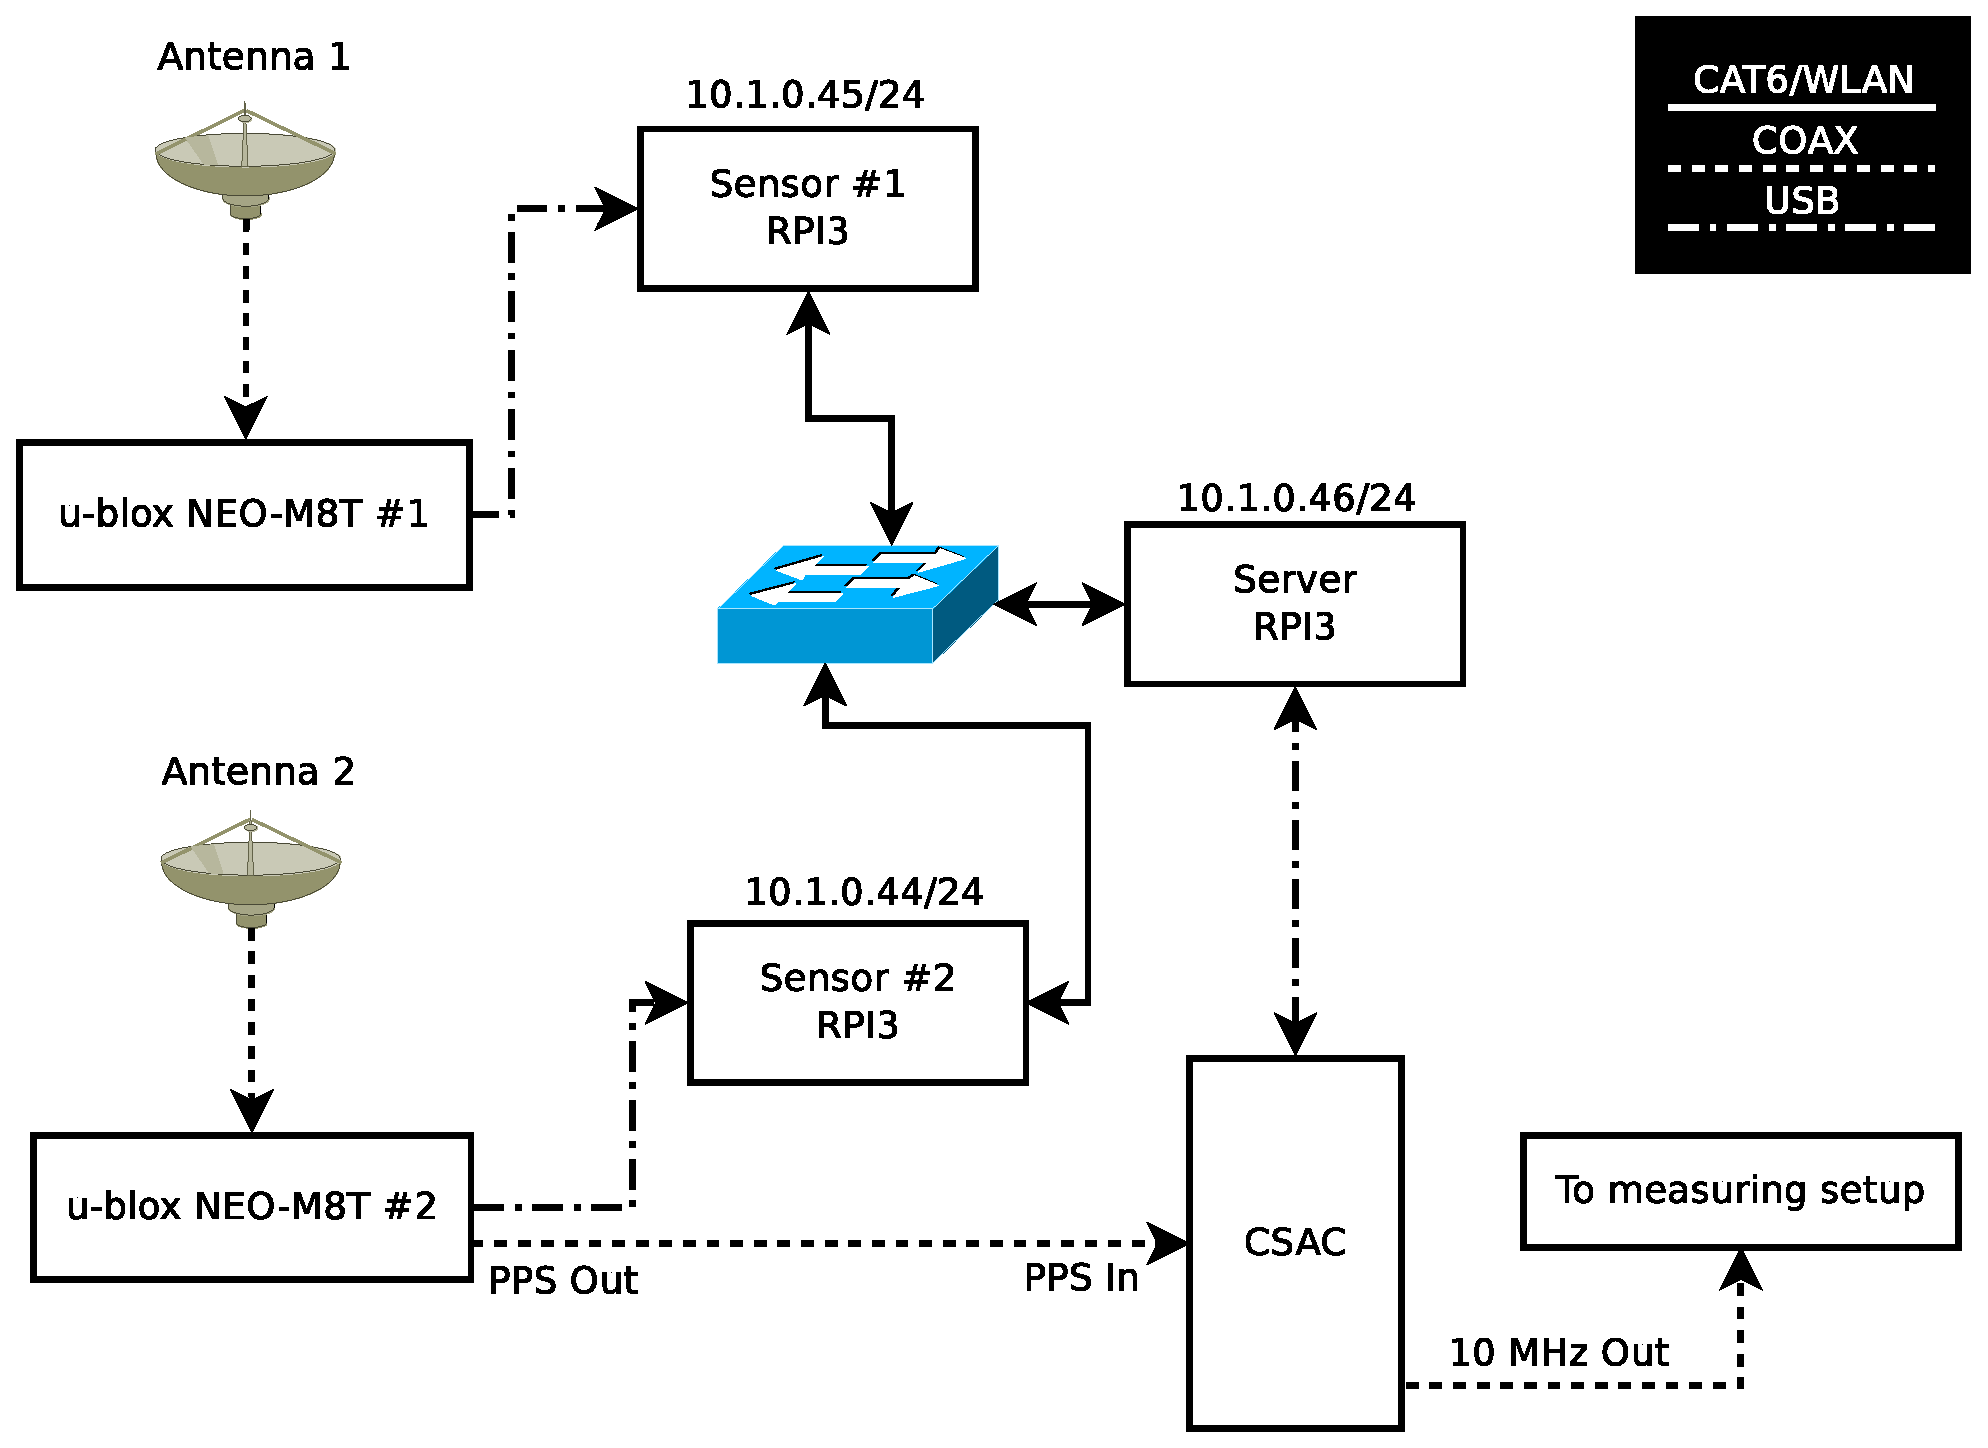
\includegraphics[scale=0.25]{thesis/graphics/server_layout.eps}
        \caption{Oppsett av server og klienter under test}
      \end{figure}
\end{frame}

\begin{frame}
\frametitle{Oppsett: måleutstyr}
  \begin{itemize}
    \item CNT-91 måler 1 PPS ut fra CSAC
    \item CNT-91 bruker 10 MHz fra tidslabb som referanse
  \end{itemize}
      \begin{figure}
        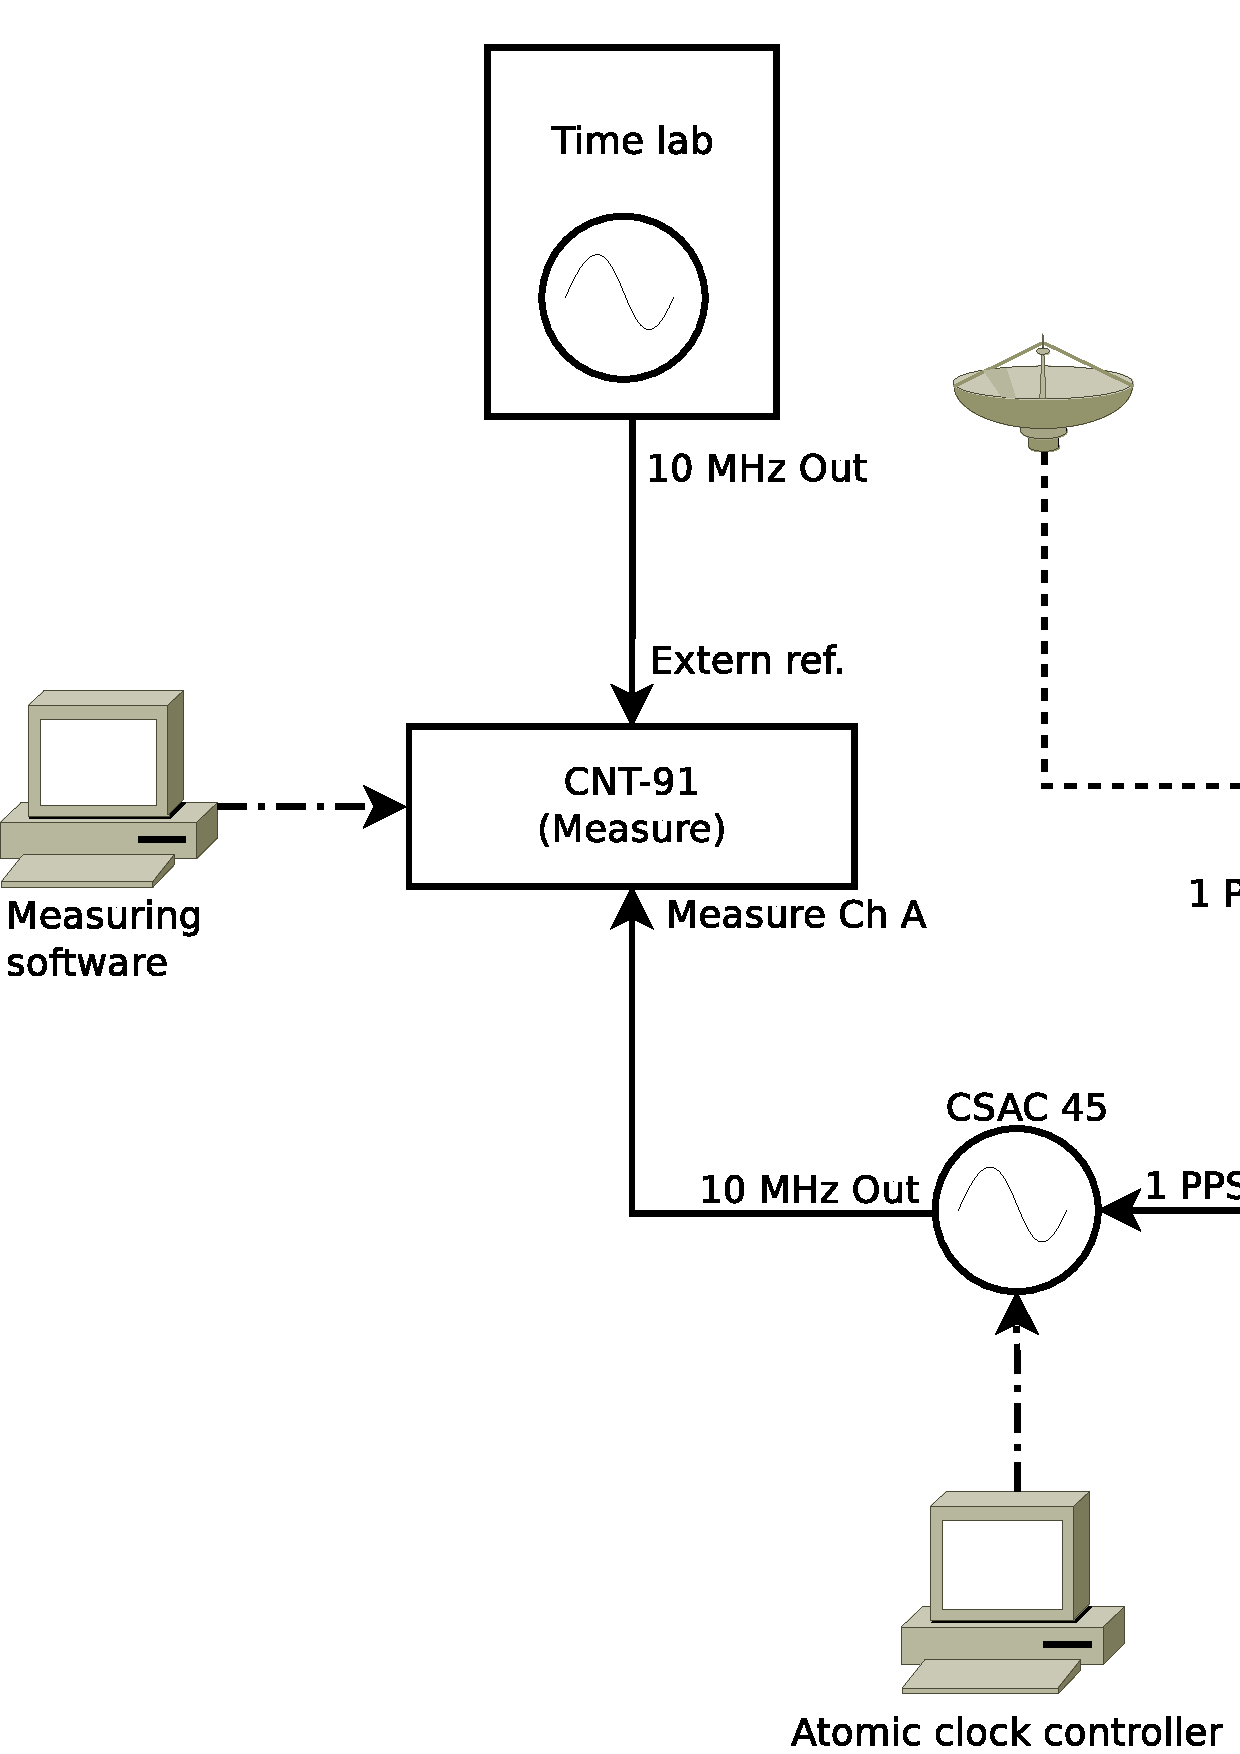
\includegraphics[scale=0.25]{thesis/graphics/measure_setup.pdf}
        \caption{Oppsett av måleutstyr}
      \end{figure}
\end{frame}

\begin{frame}
\frametitle{Oppsett: plassering av mottakere}
      \begin{figure}
        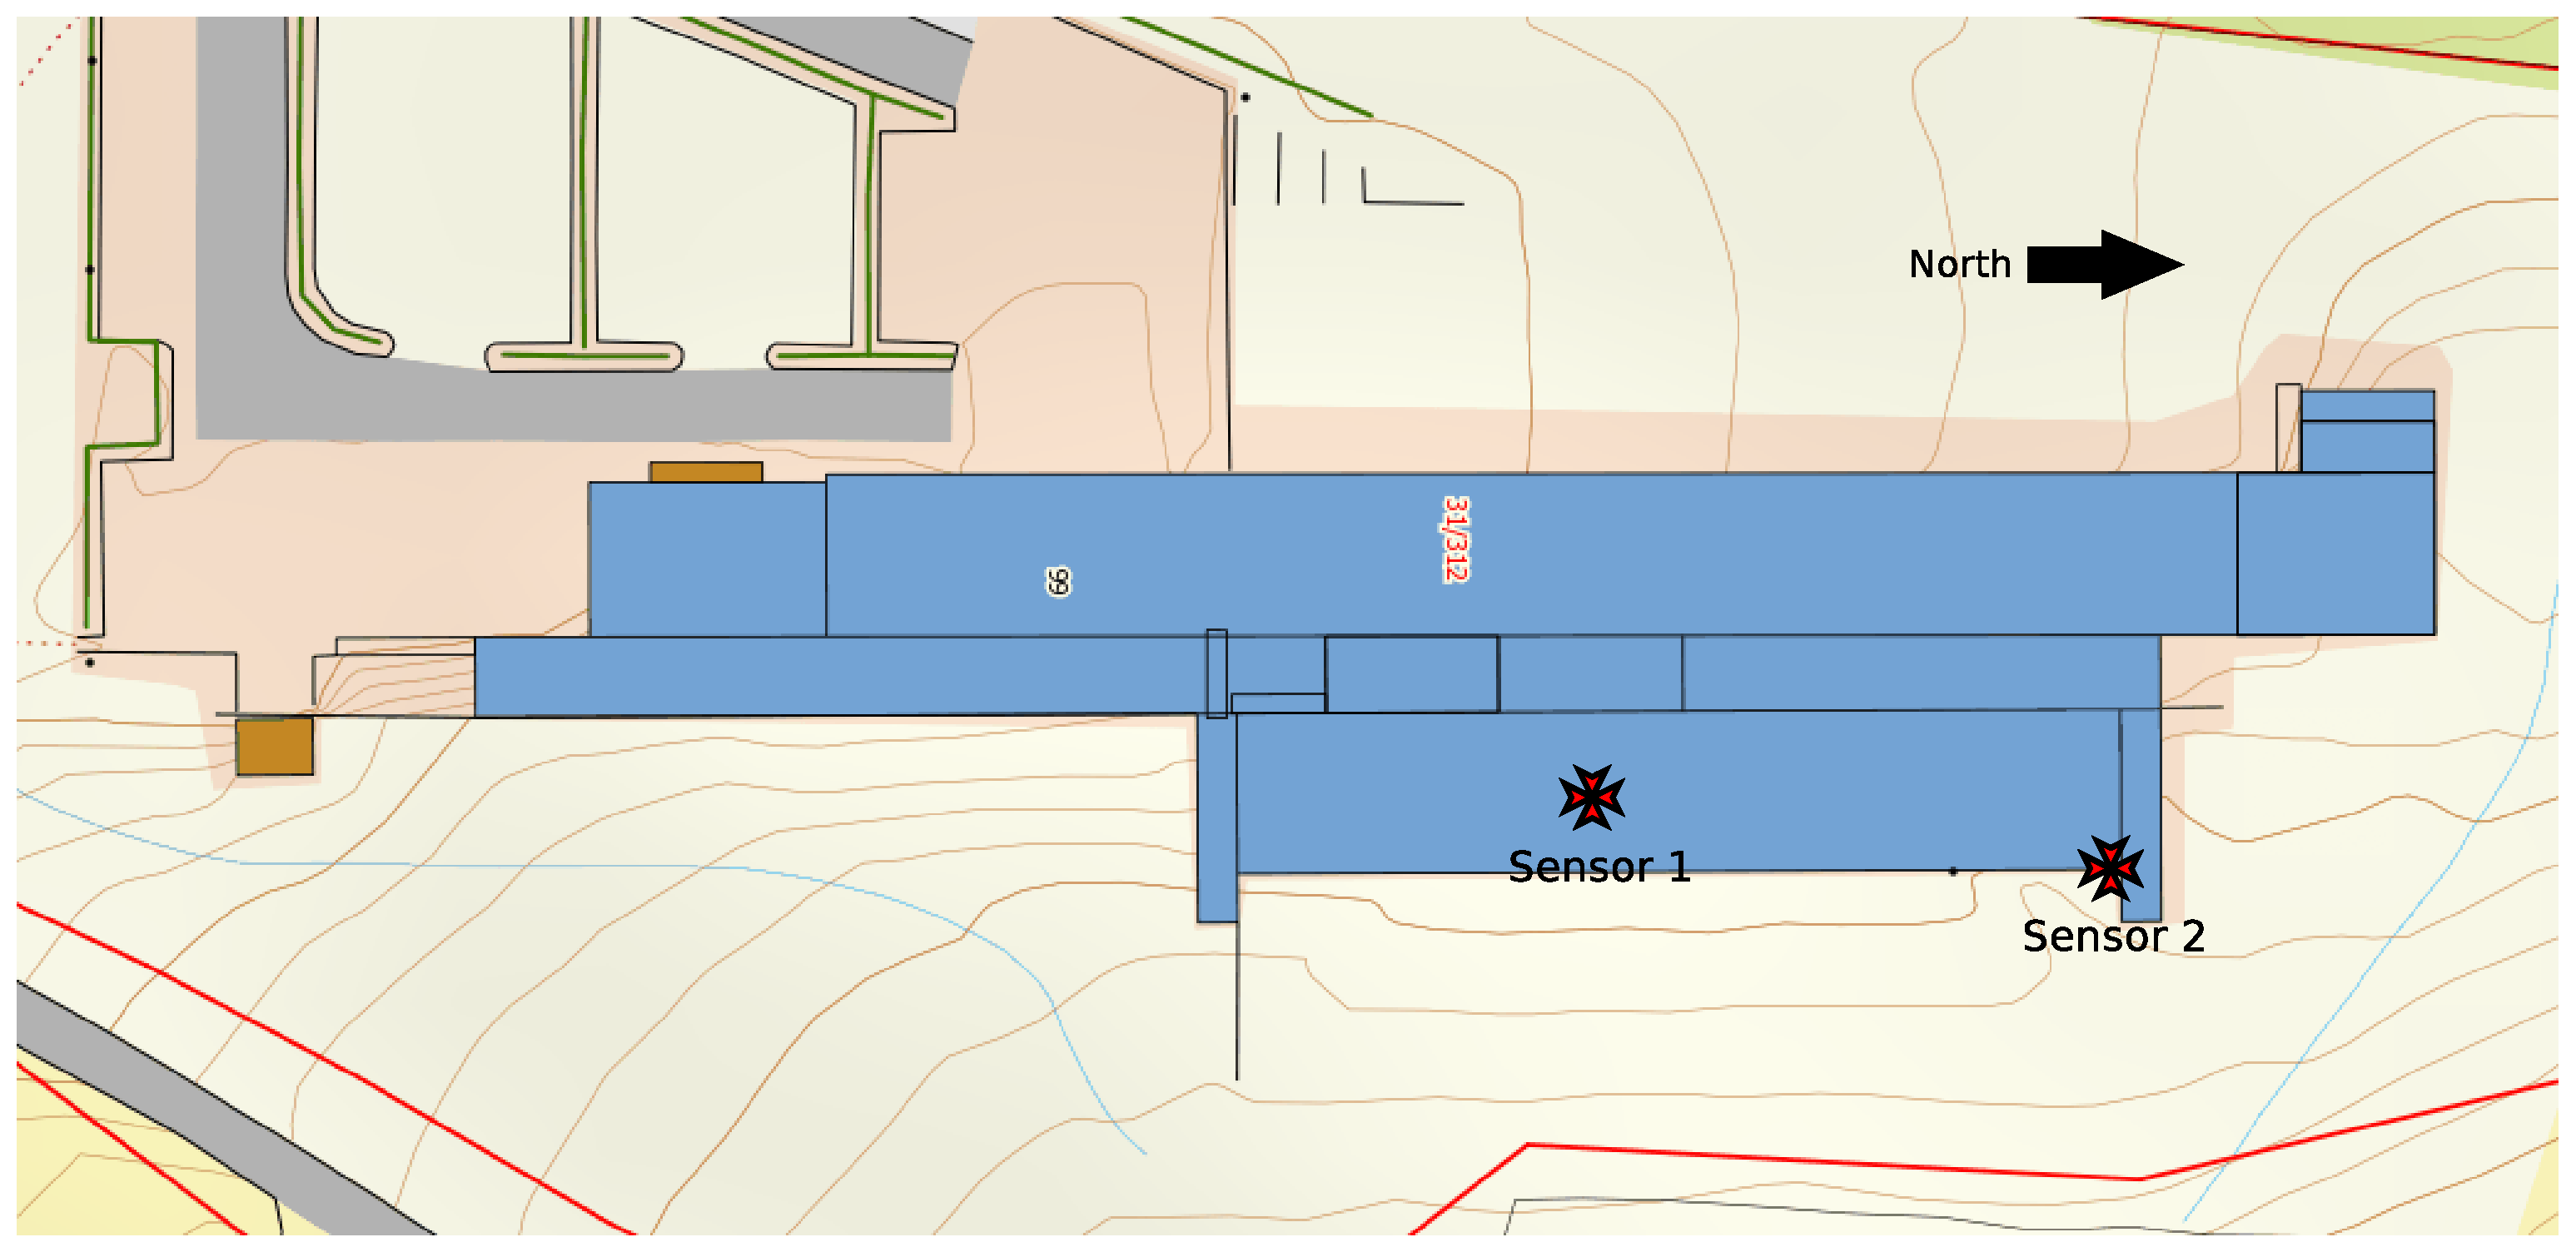
\includegraphics[scale=0.18]{thesis/graphics/roof.eps}
        \caption{Plasseringen av GPS mottakere}
      \end{figure}
\end{frame}

\begin{frame}
  \frametitle{Oppsett: grenseverdier for filter}
    \begin{table}[!htb]
      \centering
      \caption{Filter grenser}
      \label{gps_filter_table}
        \begin{tabular}{|l|l|l|}
        \hline
        \multicolumn{1}{|c|}{} & \multicolumn{1}{c|}{Sensor one} & \multicolumn{1}{c|}{Sensor two}         \\ \hline
        Altitude reference                 & 123.8$^{\circ}$ & 122.427$^{\circ}$                            \\ \hline
        Longitude reference                & 1102.1948$^{\circ}$ & 1102.1934$^{\circ}$                     \\ \hline
        Latitude reference                 & 5958.5448$^{\circ}$ & 5958.5231$^{\circ}$                     \\ \hline
        Speed reference                    & 0 knot        & 0 knot                                       \\ \hline
        Altitude deviation                 & 10$^{\circ}$        & 10$^{\circ}$                            \\ \hline
        Longitude deviation                & 0.005$^{\circ}$     & 0.005$^{\circ}$                         \\ \hline
        Latitude deviation                 & 0.005$^{\circ}$     & 0.005$^{\circ}$                         \\ \hline
        Speed deviation                    & 10 knot        & 10 knot                                     \\ \hline
        \end{tabular}
    \end{table}
\end{frame}

\begin{frame}
\frametitle{Utførelse}
  \begin{columns}
    \column{0.5\textwidth}
      \begin{itemize}
        \item Beveget antenne 1 mot antenne 2
        \item Beveget antenne 2 mot antenne 1
        \item Dekket antenne med aluminiumsfolie
        \item Noterte tid for hver handling
      \end{itemize}
    \column{0.5\textwidth}
      \begin{figure}
        \includegraphics[scale=0.20]{thesis/graphics/antenna_foil_cover.jpg}
        \caption{Antenne dekket med folie}
      \end{figure}  
    \end{columns}  
\end{frame}

\begin{frame}
\frametitle{Observasjon: GPS log}
  \subsection{Observasjon}
            \vspace{-40pt}
    \begin{columns}
      \column{0.5\textwidth}
      \begin{figure}
        \includegraphics[scale=0.40]{thesis/graphics/gnssAlt1-1.png}
      \end{figure}
                  \vspace{-30pt}
      \begin{figure}
        \includegraphics[scale=0.40]{thesis/graphics/gnssLat1-1.png}
      \end{figure}

      \column{0.5\textwidth}
      \begin{figure}
        \includegraphics[scale=0.40]{thesis/graphics/gnssLong1-1.png}
      \end{figure}
            \vspace{-30pt}
      \begin{figure}
        \includegraphics[scale=0.40]{thesis/graphics/gnssSpeed1-1.png}
      \end{figure}

    \end{columns}  
\end{frame}

\begin{frame}
\frametitle{Observasjon: Målesystem}
      \begin{figure}
        \includegraphics[scale=0.70]{thesis/graphics/cns91-and-csac-telemetry-frequency-1.png}
        \caption{Oppsett av server og klienter under test}
      \end{figure}
\end{frame}

\section{Konklusjon}
\begin{frame}
  \frametitle{Konklusjon}
\end{frame}

\section{Bibliografi}
\begin{frame}[allowframebreaks]%in case more than 1 slide needed
  \frametitle{Bibliografi}
  \printbibliography[heading=bibintoc]
\end{frame}

\end{document}